
\section{Empirical Age and Metallicity Gradients}
\label{outflows:sec:empirical}

\subsection{The Sample}
\label{outflows:sec:empirical:apogee}
There are many spectroscopic surveys to choose from to characterize the
abundance structure of the Galactic disk, such as
LAMOST~\citep{Luo2015}, GALAH~\citep{DeSilva2015, Martell2017},~\gaia-ESO
\citep{Gilmore2012}, and APOGEE\space\citep{Majewski2017}.
APOGEE is particularly well suited to this task, because it targets luminous
evolved stars accessible at large distances and observes them at near-IR
wavelengths, which are less susceptible to dust obscuration.
The disk sample is dominated by stars with Two Micron All Sky Survey
\citep{Skrutskie2006} magnitudes of~$7 < H < 13.8$ on a grid of sightlines at
Galactic latitudes of~$b = 0$,~$\pm 4^\circ$, and~$\pm 8^\circ$; targeting is
described in detail by~\citet{Zasowski2013, Zasowski2017},~\citet{Beaton2021},
and~\citet{Santana2021}.
APOGEE collects high-resolution spectra ($R \sim$ 22,500) between~$1.51$
and~$1.70~\mu$m~\citep{Wilson2019} on the 2.5 m Sloan Foundation Telescope
\citep{Gunn2006} at Apache Point Observatory and the 2.5 m du Pont
Telescope~\citep{Bowen1973} at Las Campanas Observatory, which are then
reduced and calibrated using the APOGEE data processing pipeline
\citep{Nidever2015}.
Stellar parameters such as~$T_\text{eff}$,~$\log g$, and abundances of 15 or
more elements per target star are then computed with the APOGEE Stellar
Parameters and Chemical Abundances Pipeline~\citep[ASPCAP;][]{Holtzman2015,
GarciaPerez2016}.
\par
In this chapter, we select stars from the seventeenth data
release~\citep[DR17;][]{Abdurrouf2022} that satisfy the following criteria:
\begin{itemize}

	\item \texttt{EXTRATARG == 0}

	\item \texttt{STAR\_BAD == 0}

	\item S/N~$\geq 80$

	\item $\log g = 1 - 3.8$

	\item $T_\text{eff} = 3500 - 5500$ K

\end{itemize}
To avoid contamination by the main sequence, we additionally exclude stars
with surface gravities of~$\log g > 3$ and effective temperatures of
$T_\text{eff} < 4000$ K.
These cuts yield a final sample of 191,173 red giant and red clump stars.
\par
Since one of the central interests to this chapter is to constrain the
evolution of the abundance gradient over time, we also use star-by-star ages
from~\citet{Mackereth2019b}.
Using the deep learning algorithms available through~\textsc{AstroNN}
\citep{Leung2019},~\citet{Mackereth2019b} trained a Bayesian convolutional
neural network on APOGEE spectra and asteroseismic data from the APOKASC-2
catalog~\citep{Pinsonneault2018}.
We discuss the impact of this decision
in~\S~\ref{outflows:sec:empirical:caveats} below, particularly with regard to
how this age catalog compares to the more recent~\citet{Leung2023} estimates.

\begin{figure}
\centering
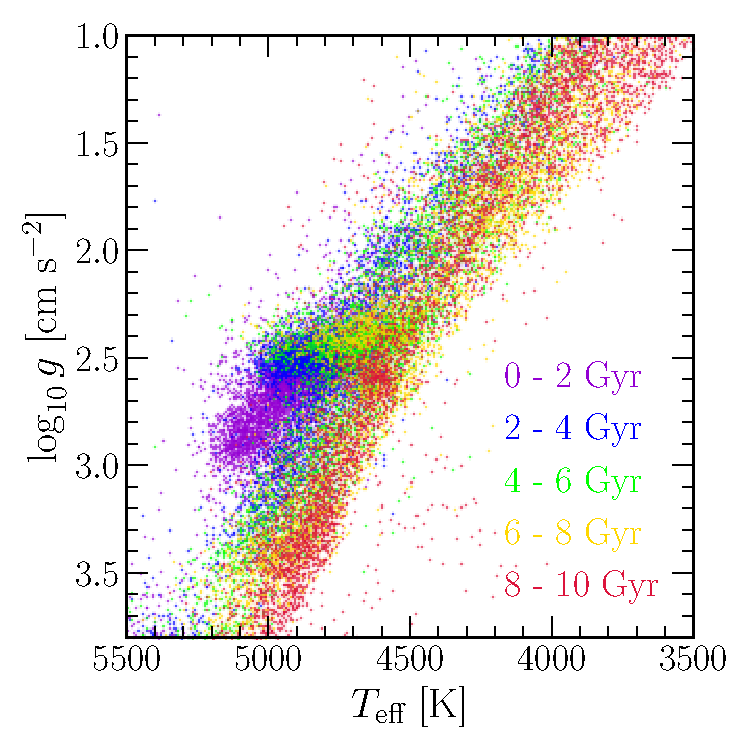
\includegraphics[scale = 0.6]{kiel_diagram.pdf}
\caption{
The Kiel diagram of our sample, color-coded by stellar age according to the
legend.
Within each age bin, we plot only a random subsample of~$N = 5000$ stars.
}
\label{outflows:fig:kiel-diagram}
\end{figure}

Fig.~\ref{outflows:fig:kiel-diagram} shows the Kiel diagram of a subsample of
our stars binned by age.
Comparing the distributions of stars along the red giant branch and red clump
between age bins indicates some systematic biases present in the sample.
The youngest stars are preferentially located in the red clump, whereas the
oldest stars distribute themselves much more evenly along the red giant branch.
This result is unsurprising as systematic uncertainties in APOGEE tend to
present as spurious correlations with~$T_\text{eff}$ and~$\log g$
\citep[e.g.,][]{Joensson2018, Eilers2022}.
However, we do not expect these systematic effects to impact our
characterizations of radial age and metallicity gradients (see discussion
in~\S~\ref{outflows:sec:empirical:caveats} below).

\afterpage{
\clearpage
\begin{landscape}
\begin{figure*}
\centering
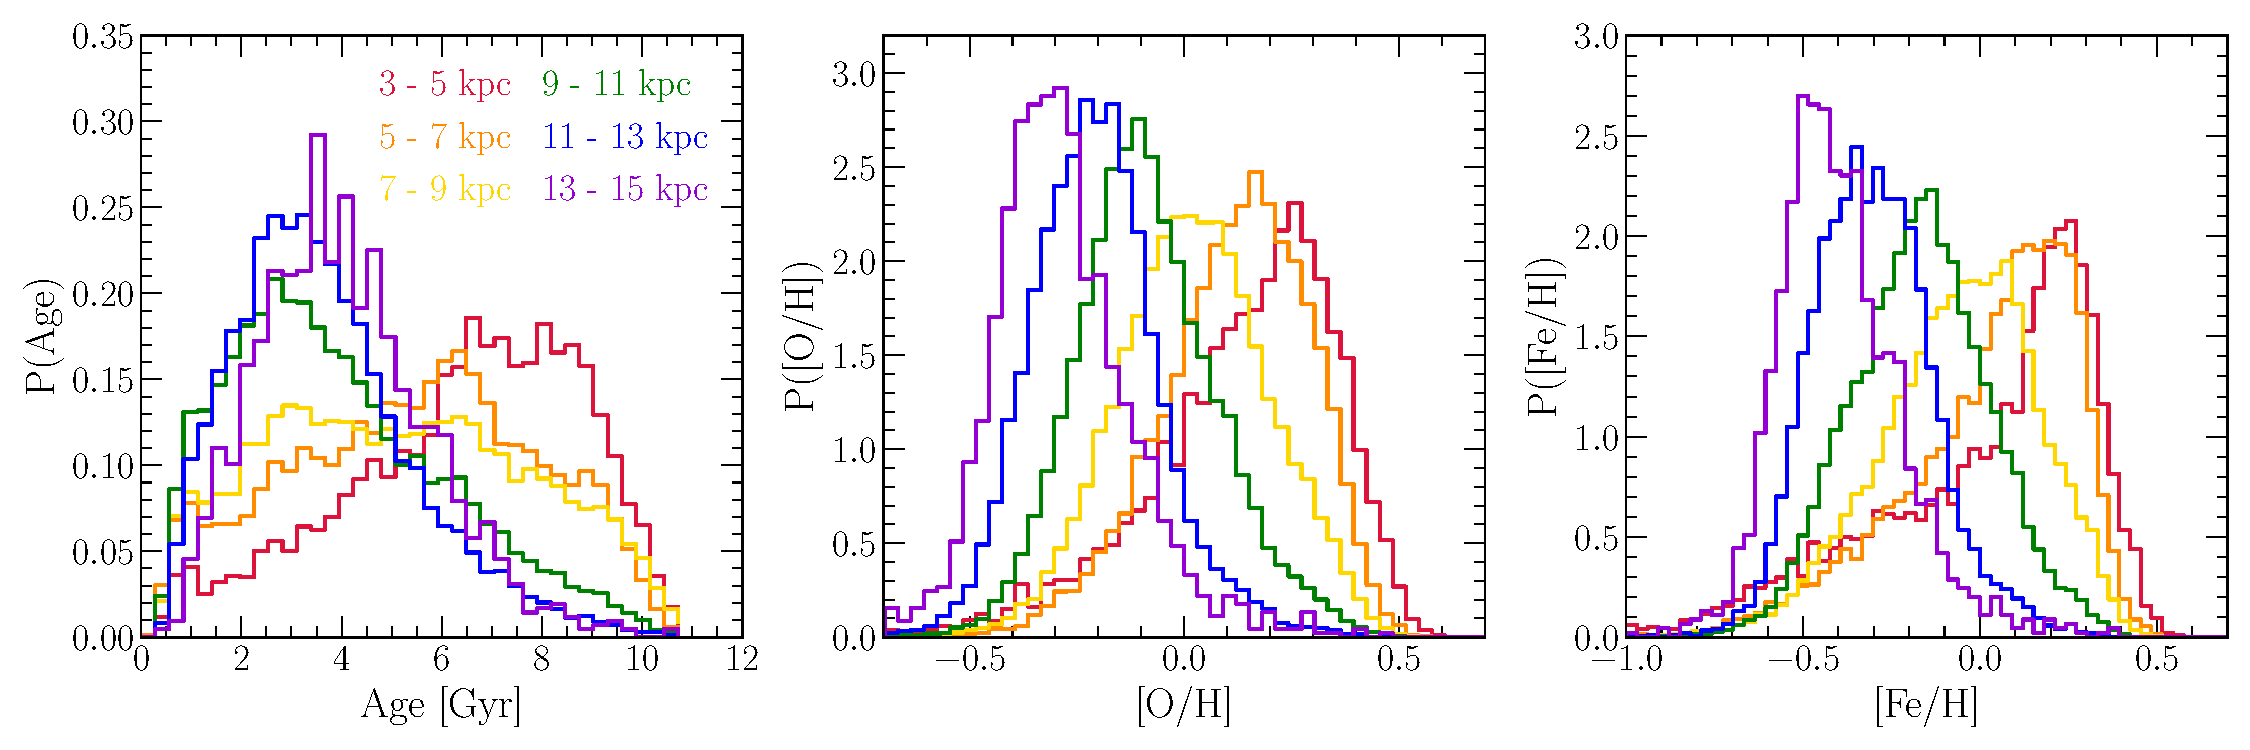
\includegraphics[scale = 0.55]{age_xh_dists.pdf}
\caption{
Age and abundance distributions from our APOGEE sample (see discussion
in~\S~\ref{outflows:sec:empirical:apogee}).
We separately compute the distributions for 2-kpc wide bins in radius indicated
by the legend in the left hand panel.
}
\label{outflows:fig:age-xh-dists}
\end{figure*}
\end{landscape}
\clearpage
}

{\color{red} Discussion of Fig.~\ref{outflows:fig:age-xh-dists} and how they
indicate the radial age and metallicity gradients.}

\subsection{Caveats}
\label{outflows:sec:empirical:caveats}
Because the~\citet{Mackereth2019b} age catalog is produced by training on APOGEE
spectra, it is possible that their estimates are biased by known trends of
abundances with stellar age (e.g., the age-[O/Fe] relation;
\citealt{Feuillet2019}).
To mitigate this potential issue,~\citet{Leung2023} take APOGEE stars with
high-cadence photometry available through~\textit{Kepler}~\citep{Borucki2010}
and compress the spectra and asteroseismic power spectra into lower dimensional
representations of themselves (i.e., a~\textit{latent space}) using a
variational encoder-decoder algorithm~\citep[e.g.,][]{LeCun2015}.
They demonstrate that this latent space contains little if any information on
chemical abundances and stellar parameters, as intended.
By augmenting the latent space with~$T_\text{eff}$ and~\feh, they are then able
to estimate ages for stars with asteroseismic power spectra predicted from
their APOGEE spectra with a modified random forest algorithm.
\par
To assess whether or not potential biases introduced by
the~\citet{Mackereth2019b} catalog impact our determination of the abundance
gradient conditioned on stellar age, we have reconducted the analysis in this
section with the~\citet{Leung2023} sample.
The results obtained with either catalog are consistent with one another,
suggesting that ages biased by abundance information in stellar spectra are not
significantly impacting our conclusions.
We have therefore focused our discussion on the~\citet{Mackereth2019b} catalog
as it offers a handful of advantages that are useful to the present chapter.
While~\citet{Mackereth2019b} infer ages for the entire APOGEE catalog,
\citet{Leung2023} only do so for the range of surface gravities spanned by
their training set ($\log_{10} g = 2.5 - 3.6$).
As a result, the sample is a factor of~$\sim$$2.5$ smaller, yielding much more
precise summary statistics in radial bins with the~\citet{Mackereth2019b}
catalog.
This decision also allows us to use luminous, low surface gravity red giants
for better coverage of the Galactic disk.
Though the~\citet{Mackereth2019b} catalog exhibits a deficit of stars at old
ages (i.e.,~$\gtrsim 10$ Gyr; see Fig.~\ref{outflows:fig:age-xh-dists} and Fig.
11 of~\citealt{Leung2023}), this should not be a problem for the present
chapter since we do not characterize the abundance gradient for such stars.

